\section{System Design}
\label{sec:design}

Motivated by the insights in \sref{sec:observations}, we propose \name, an LLM serving system built on a P/D disaggregation architecture to achieve SLO-aware and energy-efficient inference.
The following subsections detail the design of \name.



\subsection{Design Principle: A Control Theory Perspective}
\label{subsec:control}

% \jiahuan{@Minjia, need help to revise it, to remove the ``feedback''}

% \jiahuan{@Minjia, I move this paragraph from problem formulation section to here. My logic: this paragraph is to explain the difficulty of directly solving \eref{eq:formulation-freq-beg}-\ref{eq:formulation-routing-end}, which directly motivate our design (thus the ``design principle'')}

% While \eref{eq:formulation-freq-beg}-\ref{eq:formulation-routing-end} theoretically yields a global optimum, the problem is intractable to solve directly.
% The request routing (\eref{eq:formulation-routing-beg}-\ref{eq:formulation-routing-end}) is an NP-hard assignment problem~\cite{ross1975branch}.
% Moreover, the complete search space $(\{f^P_{p,k}\}, \{f^D_{d,k}\}, \mathbf{I}^P_p, \mathbf{I}^D_d)$ is too large and practically intractable.
% For online serving, the request arrival and total number $R$ are even unknown.
% Therefore, in the following sections, we simplify it from a control theory perspective and design efficient algorithms to approximate the optimum.
% \jiahuan{may remove ``from a control theory perspective'' after system design section is finalized.}

% \jiahuan{remove ``formally defines''}
% \minjia{Done. Please check other places.}
The global optimization problem in \sref{sec:formulation} defines the objective of minimizing end-to-end energy under per-phase latency SLO constraints. However, solving the problem exactly is combinatorial, and an NP-hard assignment problem~\cite{ross1975branch}, which is computationally intractable. Moreover, the future request arrivals are unknown at runtime. To make this problem tractable, we turn to a control theory perspective. Instead of solving the global problem monolithically, we observe that a P/D-disaggregated system naturally exposes two complementary control dimensions: (i) Instance-level execution configuration, which determines the latency-energy tradeoff of each prefill and decode instance. This is analogous to a local control loop in classical control system~\cite{wiener2019cybernetics}: each subsystem adjusts its internal operation point (e.g., frequency) based on its current measurable state. (ii) Assignment of incoming requests, which determines how load is distributed across instances. This corresponds directly to \emph{state-space control} in multi-subsystem systems~\cite{kalman1960general,kreindler1963contributions}: routing a request shifts an instance from one region of its state space to another, which affects both its future latency and its required operating point. 

These connections are not merely conceptual. In control theory terms, instance configuration control is a continuous, \cameraready{per-engine-iteration} control problem over a single subsystem, while routing is a discrete state-space navigation problem over multiple subsystems whose state jointly determine the global energy-latency envelop of the system. This mapping guides our design: \name applies instance-level control to continuously select energy-efficient operating points, while global routing navigates the state spaces of instances to avoid high-energy regions such as architectural tile boundaries. 

% https://www.overleaf.com/project/680d351892777cdf27140d7e#
% In \sref{sec:formulation}, we pose the energy-efficient frequency scheduling as a constrained optimization problem.
% While \eref{eq:formulation-freq-beg} - \eref{eq:formulation-routing-end} can theoretically yield a global optimum, the problem is combinatorial and NP-hard.
% In principle, many control strategies are possible, ranging from simple heuristics to complex learning-based policies.
% However, for real-world LLM serving systems, where simplicity, transparency, and responsiveness are critical, we draw inspirations from classical control policies about feedback system~\cite{wiener2019cybernetics} and state space~\cite{kalman1960general,kalman1960contributions},
% and design \textit{feedback-based} frequency control strategy (\sref{subsec:governor}) and \textit{state space navigation-based} request routing algorithm (\sref{subsec:router}).
% They operate in continuous control loops and follow the simple 3-step principle: gathering system information, doing prediction or ``what-if'' analysis, and applying new control decisions, including new frequency and routing decision.

% The primary advantage of these designs is their robustness and practicality.
% It obviates the need for potentially unreliable models for predicting request arrival times~\cite{mitzenmacher2025queueing,kakolyris2025throttll} or output lengths~\cite{stojkovic2025dynamollm,kakolyris2025throttll}, ensuring the system can generalize across dynamic workload conditions and various configurations.
% Furthermore, by avoiding complex queuing models~\cite{mitzenmacher2025queueing} or learning-based approaches~\cite{fu2024efficient,kakolyris2025throttll}, our system remains lightweight and highly interpretable, requiring only a one-time offline profiling pass to calibrate for new served models.
% \minjia{Feels redundant.}

\subsection{Overall Architecture}
\label{subsec:design-overall}

\fref{fig:overall-arch} illustrates the overall architecture of \name, which integrates three co-designed components that collectively deliver SLO-aware, energy-efficient LLM serving.

\begin{figure}[t]
    \centering
    % 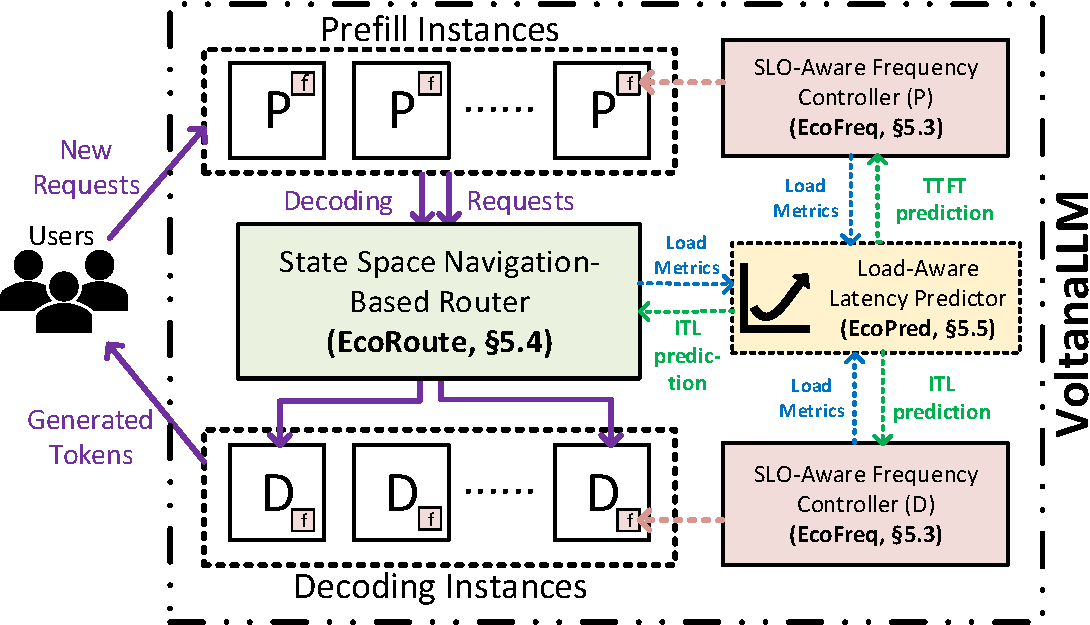
\includegraphics[width=\columnwidth]{figs/arch-new.pdf}
    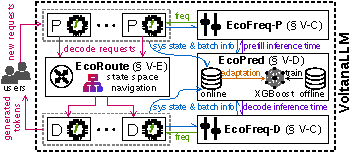
\includegraphics[width=\columnwidth]{figs/voltanallm-overall-arch.drawio.pdf}
    \caption{Overall architecture of \name. New requests are first handled by prefill instances (round-robin) to generate the first output token. \router then dispatches the requests to decode instance, from which generated tokens are streamed back to the users. \governor runs in a separate process to control the frequency of each P/D instance. \predictor provides prefill and decode model inference time predictions based on system states and batch information, while also collecting these metrics from all instances for online adaptation.}
    \label{fig:overall-arch}
\end{figure}

\noindent
\textbf{\governor} (\sref{subsec:governor}):
A phase-specific and iteration-level frequency controller for both prefill and decode instances based on current system state and batch information, maximizing energy efficiency while preserving SLO attainment. Its frequency selection is guided by the inference time predictor \predictor.

\noindent
\textbf{\predictor} (\sref{subsec:predictor}):
A accurate yet lightweight inference time predictor for both prefill and decode. Built on XGBoost~\cite{chen2016xgboost}, it combines both offline profiling and online adaptation to maintain accuracy under workload dynamics and mitigates distribution shift between offline and online data.

\noindent
\textbf{\router} (\sref{subsec:router}):
An energy-efficient router that assigns prefill-generated requests to decode instances.
It mitigates architectural granularity-induced energy inefficiency (\sref{subsec:tile-effect}) by analyzing and navigating each decode instance state spaces before making routing decisions, avoiding unnecessary transition into high-frequency regions.
% It also relies on accurate latency predictions from \predictor.


% \begin{enumerate}
%     \item \governorfull \newline(\textbf{\governor}): A feedback-based frequency controller that performs frequency scaling in a lightweight, phase-specific, and fine-grained (per-iteration) manner, to maximize energy efficiency while preserving SLO attainment. Its decisions are guided by real-time load metrics and latency predictions from \predictor.
%     \item \routerfull (\textbf{\router}): A router specifically designed for prefill-to-decode request routing. It mitigates boundary-induced energy inefficiency by analyzing and navigating in the state spaces of decode instances. It also relies on accurate ITL predictions from \predictor.
%     \item \predictorfull (\textbf{\predictor}): A lightweight yet accurate TTFT/ITL predictor. It utilizes collected profiling data and interpretable linear regression to estimate latencies.
% \end{enumerate}

% \begin{enumerate}
%     % \item \jiahuan{TODO: fix linewidth problem}
%     \item \governorfull \newline(\textbf{\governor}): A feedback-based frequency controller that performs frequency scaling in a lightweight, phase-specific, and fine-grained (per-iteration) manner, to maximize energy efficiency while preserving SLO attainment. Its decisions are guided by real-time load metrics and latency predictions from \predictor.
%     \item \routerfull (\textbf{\router}): A router specifically designed for prefill-to-decode request routing. It mitigates boundary-induced energy inefficiency by analyzing and navigating in the state spaces of decode instances. It also relies on accurate ITL predictions from \predictor.
%     \item \predictorfull (\textbf{\predictor}): A lightweight yet accurate TTFT/ITL predictor. It utilizes collected profiling data and interpretable linear regression to estimate latencies.
% \end{enumerate}







\subsection{\governor: SLO-Aware and Iteration-Level Frequency Control for Responsive Energy Adaptation} 
\label{subsec:governor}

% Although modern GPUs are capable of dynamic frequency scaling, leveraging it for energy-efficient LLM serving is non-trivial.
% First, the inherent energy-latency trade-off (\sref{sec:obs-u-shape}) demands a control policy that is both adaptive to real-time workload and capable of ensuring SLO attainment.
% Second, temporal variations in P/D demands (\sref{subsec:temporal-variation}) necessitate phase-specific policies which are able to operate each phase at its distinct optimal frequency.
% \jiahuan{TODO: sync it with observation section}
% Third, frequency adjustment itself introduces non-negligible overhead. 
% As reported in \cite{stojkovic2025dynamollm}, invoking frequency changes via blocking \texttt{nvidia-smi} calls incurs an overhead of $\sim$50ms, which is prohibitively expensive within the latency-sensitive engine loop.

Although modern GPUs (e.g., NVIDIA A100/H100) expose APIs to set frequencies, they do not tune frequencies dynamically in response to load~\cite{vspetko2021dgx}.
As such, using them effectively for SLO-aware and energy-efficient LLM serving is non-trivial due to two challenges.
First, temporal variations in P/D demands (\sref{subsec:temporal-variation}) require distinct frequency policies for each phase, as they exhibit different optimal operating points depending on the workload.
The inevitable energy-latency trade-off (\sref{sec:obs-u-shape}) also requires a control policy that adapts to real-time workload variations while guaranteeing SLO attainment.
Second, coarse-grained frequency adjustment is ineffective in handling rapid iteration-level dynamism in workloads (\sref{subsec:temporal-variation}), yet existing fine-grained frequency control introduces expensive overhead.
Recent studies report $\sim$50 ms latency per change via blocking \texttt{nvidia-smi} commands\cite{stojkovic2025dynamollm}, which is unsuitable for latency-sensitive engine loops where each generation step typically completes within tens to hundreds of milliseconds.


To overcome these challenges, we design \governor, a responsive, SLO-aware controller that performs iteration-level GPU frequency adjustment for both prefill and decode instances. 
\fref{fig:governor-exec-flow} illustrates how \governor interacts with P/D instances.
To overcome the overhead of frequency settings via \texttt{nvidia-smi}, \governor introduces multiple optimizations.
It runs as a \textit{independent} process outside the critical inference path \cameraready{to completely hide the switching overhead}, communicating with the inference engine via low-overhead ZeroMQ~\cite{zeromq}. 
% \minjia{Add the main benefit of using ZeroMQ, reduced communication overhead? Overlapping of freq control function call and inference execution?}
% \jiahuan{fixed, add ``for low-overhead communication''}
Rather than expensively setting frequency via \texttt{nvidia-smi}, \governor leverages \texttt{nvmlDeviceSetGpuLockedClocks} API from NVIDIA Management Library~\cite{nvml} to apply new frequency \cameraready{at the whole-GPU granularity}.
Our measurements show it consumes $<$3 ms.
Upon scheduling a new batch, the inference engine sends its current batch information $\mathbf{B}$ and system state $\mathbf{M}$ to \governor.
\governor then selects an appropriate GPU frequency and applies it immediately. 
This per-iteration loop enables responsive adaptation to instantaneous workload conditions.
Furthermore, the frequency selection algorithm (we will discuss it later) executes in $\sim$0.5 ms.
The total end-to-end overhead of \governor per iteration is thus $<$4 ms and is overlapped with the engine's model inference.
Consequently, although the beginning of an inference step may use the previous iteration's frequency, this period is negligible compared to the total model inference time (e.g., 500 ms for prefill and 50 ms for decode), introducing negligible control inaccuracy.
This lightweight design achieves per-iteration responsiveness to workload variations with negligible overhead, enabling \governor to apply \cameraready{per-engine-iteration}, independent control for each phase and instance, 
thereby maximizing energy savings while ensuring SLO attainment.
% \jiahuan{actually, the execution of \governor is overlapped with model inference, as shown in \fref{fig:governor-exec-flow}. We choose this design because it takes significantly shorter time than the model inference, i.e., although the start part of the model inference use the old frequency, this part is very small and negligible. I correct the description in this paragraph.}

% To overcome the overhead of frequency settings via \texttt{nvidia-smi}, \governor applies \texttt{nvmlDeviceSetGpuLockedClocks} API from NVIDIA Management Library~\cite{nvml} to apply new frequency.
% Our measurements shows it consumes $<$3ms.
% Furthermore, the inference time predictors $T_P(\cdot)$ and $T_D(\cdot)$ takes $\sim$0.5ms to execute each time.
% Thus, the total end-to-end overhead of \governor per engine iteration is $<$4ms, which is significantly shorter than the typical model inference time for prefill ($\sim$500ms) and decode ($\sim$50ms).

\begin{figure}[!t]
    \centering
    % 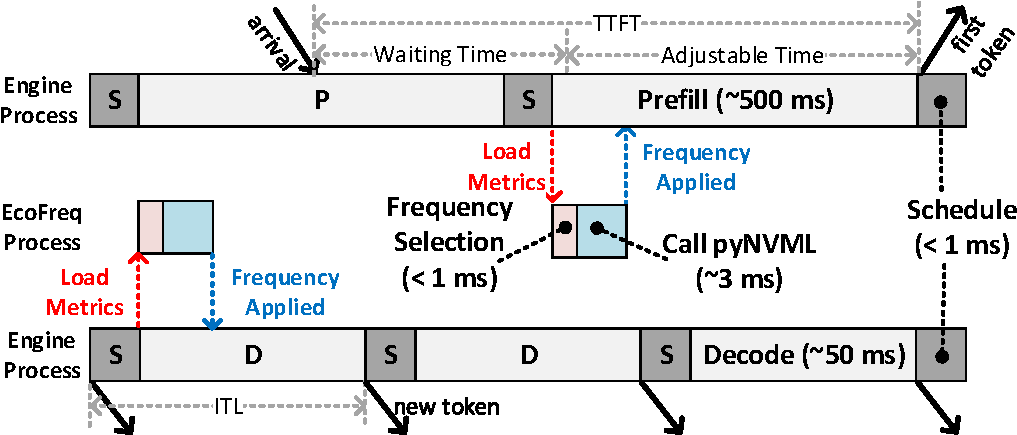
\includegraphics[width=\columnwidth]{figs/pd-flow.pdf}
    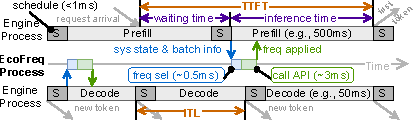
\includegraphics[width=\columnwidth]{figs/voltanallm-governor.drawio.pdf}
    \caption{Execution flow of \governor with P/D instances. \governor runs as a separate lightweight process that collects system states and batch  from the engine and performs sub-millisecond iteration-level frequency control.}
    \label{fig:governor-exec-flow}
\end{figure}

The following steps details the SLO-aware, phase-specific frequency selection algorithm of \governor (\aref{alg:ecofreq}).
Let $\mathcal{F}$ be the set of frequency options.
Each invocation of \governor comprises three steps:
\ding{202} \textbf{Queue Check} (\alref{algline:step1-beg}-\ref{algline:step1-end}):
If there are requests in \emph{waiting} state (queued requests awaiting scheduling), 
% \minjia{It feels confusing to use terms like waiting state, running state without first introducing a state diagram or control model yet.}
% \jiahuan{we should introduce this in the background section. Space is enough}
% \minjia{I addressed it by adding a short phrase explaining each state. Let me know if that makes it clearer.}
% \jiahuan{LGTM}
\governor selects the highest frequency $\max(\mathcal{F})$ to promptly clear waiting requests and prevent SLO violations due to queue buildup. 
This prevents a scenario where a lower frequency, while sufficient for \emph{running} (actively executing decode steps) request SLOs, would reduce overall throughput, causing waiting requests to accumulate and subsequently violate their SLOs.
\ding{203} \textbf{Phase-Specific Adjustment} (\alref{algline:step2-beg}-\ref{algline:step2-end}):
The target token latency for each phase can be decomposed as:
\begin{equation}
    \text{Latency} = T_{\text{fixed}} + T_{\text{inference}}(f) \le \text{SLO}
\end{equation}
where $T_{\text{fixed}}$ is frequency-\emph{irrelevant} time (e.g., request scheduling and waiting) and $T_{\text{inference}}(f)$ is the frequency-\emph{dependent} GPU model inference time.
As shown in \fref{fig:governor-exec-flow}, $T_{\text{fixed}}$ differs by phase.
For \emph{decode}, $T_{\text{fixed}}$ is negligible scheduling time ($<$1ms).
Conversely, for \emph{prefill}, $T_{\text{fixed}}$ is primarily the request's waiting time (i.e., from arrival to being scheduled for running), which is non-negligible.
Since frequency scaling only controls $T_{\text{inference}}(f)$, \governor sets a phase-adjusted target $S$ for $T_{\text{inference}}(f)$ to ensure SLO attainment:
\begin{equation}
    T_{\text{inference}}(f) \le S = \begin{cases}
        S_P - \max\left( \mathbf{T}_{\text{waiting}} \right), & \text{prefill,} \\
        S_D, & \text{decode,}
    \end{cases}
\end{equation}
where $S_P$ and $S_D$ are TTFT and ITL SLOs, respectively, and $\max\left( \mathbf{T}_{\text{waiting}} \right)$ is the maximum waiting time among requests within a prefill batch.
\ding{204} \textbf{Frequency Selection} (\alref{algline:step3-beg}-\ref{algline:step3-end}):
Using the prefill ($T_P(\cdot)$) or decode ($T_D(\cdot)$) inference time predictors, \governor iterates through candidate frequencies $\mathcal{F}$ in ascending order, choosing the lowest frequency that makes $T_{\text{inference}}(f) \le S$.
If none meets the target, it defaults to $\max(\mathcal{F})$ to preserve SLO attainment.
The predictors $T_P(\cdot)$ and $T_D(\cdot)$ take $\sim$0.5 ms to execute each time.
We achieve this through careful model selection (discussed in \sref{subsec:predictor}), which enables per-iteration frequency selection of \governor.

% \jiahuan{add sentences to emphasize the small total overhead}

% \begin{figure}[!ht]
%     \centering
%     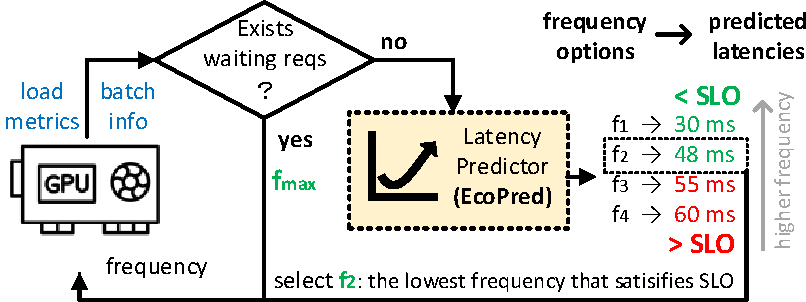
\includegraphics[width=\columnwidth]{figs/ecofreq.pdf}
%     \caption{
%     Algorithm of \governor to select frequency. 
%     SLO and list of frequency options are given when deploy \name.
%     Inputs are load metrics and batch information from the engine.
%     Output is the selected frequency.
%     \jiahuan{redraw figure, add steps}
%     }
%     \label{fig:governor-arch}
% % \end{figure}

\begin{algorithm}[!t]
% \caption{\governor: SLO-Aware and Iteration-Level Frequency Selection}
\caption{\governor: SLO-Aware Frequency Selection}
% \minjia{This algorithm only shows how to select frequency but it does not show how it performs control, e.g., where this control is placed? You may need to add the inference step loop and add the control right before the call of the decoding step.}
% \jiahuan{my idea is, this is just the frequency selection algorithm, \fref{fig:governor-exec-flow} shows the control process. I believe it is more clear. Is it OK?}
% \minjia{Yes.}
 \label{alg:ecofreq}
 \begin{algorithmic}[1]

    \Require Current system status $\mathbf{M}$, batch information $\mathbf{B}$, frequency option list $\mathcal{F}$, model inference time predictors $T_P(\cdot)$ and $T_D(\cdot)$, TTFT SLO $S_P$, ITL SLO $S_D$.
    
    \Ensure Selected GPU frequency $f$.

    \If{$\Call{HasWaitingReqs}{\mathbf{M}}$}  \Comment{\textbf{step \ding{202} Queue check}} \label{algline:step1-beg}
        \State \Return $\max(\mathcal{F})$ \Comment{clear backlogged reqs timely}
    \EndIf \label{algline:step1-end}

    \If{$\Call{IsPrefill}{\mathbf{B}}$} \Comment{\textbf{step \ding{203} Phase adjustment}} \label{algline:step2-beg}
        \Statex /* prefill: deduct the waiting time from SLO budget */
        \State $S \gets S_P - \max( \mathbf{T}_{\text{waiting}}(\mathbf{B}) )$, $T_{\text{inference}}(\cdot) \gets T_P(\cdot)$ 
        % \State $T_{\text{inference}}(\cdot) \gets T_P(\cdot)$
    \Else
        \State $S \gets S_D$, $T_{\text{inference}}(\cdot) \gets T_D(\cdot)$ \Comment{/* decode */}
    \EndIf \label{algline:step2-end}

    % \State $f^\star = \argmin_{f\in\mathcal{F}} T_{\text{inference}}(\mathbf{M}, \mathbf{B}, f) \le S$
    % \If 

    % \State $f^\star = \argmin_{f\in\mathcal{F}} T_{\text{inference}}(\mathbf{M}, \mathbf{B}, f) \le S$ \Comment{\textbf{step \ding{204} Frequency selection}} \label{algline:step3-beg}
    % \If{$f^\star \ne \emptyset$} 
    %     \State $f^\star = \max(\mathcal{F})$ \Comment{no freq can meet SLO, return max}
    % \EndIf
    

    \For{$f \in \sorted(\mathcal{F})$}  \Comment{\textbf{step \ding{204} Frequency selection}} \label{algline:step3-beg}
        \If{$T_{\text{inference}}(\mathbf{M}, \mathbf{B}, f) \le S$}
            \State \Return $f$ \Comment{minimum frequency to meet the SLO}
        \EndIf
    \EndFor

    \State \Return $\max(\mathcal{F})$  \Comment{no freq can meet SLO, return max} \label{algline:step3-end}

 \end{algorithmic}
\end{algorithm}


% \begin{algorithm}[!t]
%     \linespread{1}\selectfont
%     \caption{\governor: SLO-Aware Freq. Selection}
%     \label{alg:ecofreq}
%     \KwIn{Current system status $\mathbf{M}$, batch information $\mathbf{B}$, frequency option list $\mathcal{F}$, model inference time predictors $T_P(\cdot)$ and $T_D(\cdot)$, TTFT SLO $S_P$, ITL SLO $S_D$.}
%     \KwOut{Selected GPU frequency $f$.}

%     % Step 1
%     \If{$\mathrm{HasWaitingReqs}(\mathbf{M})$ \tcp*[h]{Step \ding{202} Queue check}}{   \label{algline:step1-beg}
%         \Return $\max(\mathcal{F})$ \tcp*[r]{clear backlogged reqs timely}   \label{algline:step1-end}
%     }

%     % Step 2
%     \tcp{Step \ding{203} Phase adjustment}
%     \eIf{$\mathrm{IsPrefill}(\mathbf{B})$}{
%         \tcp{prefill: deduct the waiting time from SLO budget}
%         $S \gets S_P - \max( \mathbf{T}_{\text{waiting}}(\mathbf{B}) )$, $T_{\text{inference}}(\cdot) \gets T_P(\cdot)$\;
%     }{
%         $S \gets S_D$, $T_{\text{inference}}(\cdot) \gets T_D(\cdot)$ \tcp*[r]{decode}
%     }

%     % Step 3
%     \tcp{Step \ding{204} Frequency selection}
%     \ForEach{$f \in \mathrm{sorted}(\mathcal{F})$}{
%         \If{$T_{\text{inference}}(\mathbf{M}, \mathbf{B}, f) \le S$}{
%             \Return $f$ \tcp*[r]{min frequency to meet the SLO}
%         }
%     }

%     % Fallback
%     \Return $\max(\mathcal{F})$ \tcp*[r]{no freq can meet SLO, return max}

% \end{algorithm}


% The whole algorithm is lightweight and takes $<$ 1 ms to finish.


% \jiahuan{revising}

% The new frequency is then applied via pyNVML (\textasciitilde 3 ms), avoiding the high overhead of \texttt{nvidia-smi}.
% Because the entire control cycle (<4 ms) is significantly shorter than the typical model execution time of both prefill (\textasciitilde 500 ms) and decode iteration (\textasciitilde 50 ms), our approach achieves per-iteration responsiveness with negligible performance overhead.

% Upon scheduling a new batch, the engine sends the relevant batch metadata $\mathbf{B}$ and system status $\mathbf{M}$ to \governor.
% The controller then performs its frequency selection algorithm.
% The new frequency is then applied to the GPU.


% via pyNVML (\textasciitilde 3 ms), avoiding the high overhead of \texttt{nvidia-smi}.


% First, the inherent trade-off between energy and latency (\sref{sec:obs-u-shape}) requires a control policy that is both adaptive to real-time load and meticulously managed to prevent SLO violations.\

% Furthermore, temporal variation of P/D demands (\sref{subsec:temporal-variation}) necessitates the phase-specific control policy that allows each phase to operate at its distinct optimal point.

% Third, a major obstacle is the non-negligible overhead of frequency setting itself. 
% Recent studies such as DynamoLLM~\cite{stojkovic2025dynamollm} report that invoking frequency changes via blocking \texttt{nvidia-smi} calls incurs $\sim$50 ms of overhead per iteration, which is expensive in latency-sensitive engine loop.


% To mitigate this overhead, existing methods propose window-based approach by enlarging the control granularity (e.g., 5 seconds), but such coarse granularity lacks the necessary responsiveness for batch sizes that can fluctuate rapidly, especially for the prefill phase (\sref{subsubsec:ablation-responsiveness}).

% \jiahuan{simplify this paragraph}
% To address these challenges, we introduce \governor, a module that dynamically adjusts the GPU frequency in an SLO-aware, phase-specific, and lightweight manner.
% % Critically, it executes asynchronously to reduce the frequency control overhead while maintaining the responsiveness required for per-iteration adjustments.
% \fref{fig:governor-exec-flow} shows how \governor works with engine iterations of both P/D phases.
% It runs in a separate process to avoid potential overhead, and communicate with the engine via ZeroMQ~\cite{noauthor_zeromq_nodate}, a high performance IPC framework.
% % To prevent data staleness, the ZeroMQ queue size is set to 1.
% Upon scheduling a new batch, the engine sends the relevant metadata and load metrics to the controller.
% The controller then performs its frequency selection logic (<1 ms).



% A key difference between P/D phases is how the controller accounts for waiting time.
% As illustrated in \fref{fig:governor-exec-flow}, the TTFT of a prefill request contains two parts:  \textit{waiting time} and \textit{execution time} (which can be adjustable via frequency).
% Therefore, to meet the TTFT SLO, \governor subtracts the waiting time from total SLO budget, and use subtraction result as the target of frequency selection.
% This consideration is not applied for the decode phase, as new tokens are generated auto-regressively without any extra waiting time.

% \fref{fig:governor-arch} details the frequency selection algorithm of the \governor.
% It selects frequency from a list of frequency options, which are adjustable parameters when deploying \name.
% The design is a feedback-based, stateless decision procedure whose inputs are system load metrics and batch information.
% The algorithm begins by checking the waiting queue; if a backlog exists, it directly selects themaximum frequency as algorithm output.
% Otherwise, if the queue is clear, it performs the latency prediction: for all candidates in the list of frequencies, it queries \predictor using frequency, system load metrics and batch information, and get a list of predicted latencies.
% Finally, it selects the lowest frequency in the list whose corresponding predicted latency satisfies the SLO target, and uses it as the algorithm output.
% The whole algorithm is lightweight and takes $<$ 1 ms to finish.



% \fref{fig:governor-arch} shows the algorithm how \router selects the frequency.
% It selects frequency from a list of frequency options, which are adjustable when deploying \name.
% Overall it is a feedback-based decision logic, running as a stateless procedure.
% The algorithm inputs are system load metrics and batch information.
% It first performs waiting queue check: if there exist requests in the waiting queue, the algorithm returns maximum frequency ($f_{\max}$) as the output to clear backlog and prevent starvation.
% Otherwise, for all frequency candidates, it queries \predictor using input metrics to get predicted latencies of all frequency candidates.
% Then, it selects the lowest frequency whose predicted latency satisfies the SLO target.
% This selected frequency is the output of algorithm.

% the feedback control loop of \governor.
% Given a latency predictor and a list of frequency options which are set when deployment, it works in a stateless way.
% During each 
% First, to prevent starvation, if there are waiting requests in the queue, it immediately switches to the maximum frequency to clear the backlog as quickly as possible.
% Otherwise, it queries \predictor (see \sref{subsec:predictor} for details) to predict the TTFTs/ITLs for the current iteration batch under each potential frequency option, and selects the lowest one that satisfies the SLOs as targeted frequency.
% \jiahuan{TODO}
% \jiahuan{TODO: maybe need to refine}
% \minjia{This is a bit abrupt. The whole section is primarily dedicated to explaining how the frequency scaling can be made lightweight. It lacks "how" to use this lightweight, fine-grained per-iteration frequency control for energy saving. You may need to refer to Figure 7 and expand the caption to provide more details. For example, you can first define the state of frequency (e.g., either high-low, or a list), and then say that we view it as a 0-step markov decision process (the one we discussed on slack), and the controller piggybacks on the LLM decoding loop and at each step it takes actions (e.g., check the waiting queue, query the \predictor, and select a frequency from the list to meet the SLO).   }








The effectiveness of \governor relies on the accurate model inference time predictors $T_P(\cdot)$ and $T_D(\cdot)$ under varying system states and GPU frequencies.
To achieve this, we design online-adaptive predictors \predictor built on XGBoost~\cite{chen2016xgboost}, a model widely adopted for its ability to model performance while remaining lightweight and robust to feature interactions~\cite{chen2018tvm,chen2018learning}.
\predictor combines \emph{offline profiling} with \emph{online adaptation} to remain accurate under dynamic workloads.
% \minjia{Let's call it online adaptation instead of online fine-tuning.}
% \jiahuan{LGTM}

\noindent
\textbf{Rationale: predictability and feature selection.}
For offline analysis, we perform the same profiling as in \sref{sec:obs-u-shape} but collect additional system state metrics: number of running requests (i.e., batch size) $N_{\text{req}}$, batched token number $N_{\text{tok}}$, and token number in KV cache storage $N_{\text{kv}}$.
\fref{fig:pred-tile} shows an example of profiling results for LLaMA-3.1-8B on A100.
The results clearly demonstrate that model inference time exhibits strong predictability under varying GPU frequencies and system states.
For prefill, inference time shows a strong linear relationship with $N_{\text{tok}}$. Conversely, decode inference time exhibits the ``staircase'' effect (as discussed in \sref{subsec:tile-effect}), yet remains highly predictable from $(N_{\text{req}}, N_{\text{kv}})$ within each tile.
These observations are formalized as:
\begin{align}
    T_P \left(\mathbf{M}, \mathbf{B}, f \right) \approx & a_f \cdot N_{\text{tok}} + b_f, \label{eq:pred-ttft} \\
    T_D \left( \mathbf{M}, \mathbf{B}, f  \right)  \approx & c_f \cdot N_{\text{req}} + d_f \cdot N_{\text{kv}} + e_f\ \ (\text{each tile}). \label{eq:pred-itl}
\end{align}
This predictability reflects the distinct computational characteristics of two phases.
For the compute-bound prefill phase, total computation theoretically scales linearly with the batched token number $N_{\text{tok}}$~\cite{vaswani2017attention,dao2023flashattention2}, yielding the highly linear relationship in \fref{fig:pred-ttft}.
In contrast, for the decode phase, $N_{\text{req}}$ determines the GEMM computational load~\cite{vaswani2017attention}, while $N_{\text{kv}}$ dictates the Attention layer computation and KV cache memory access~\cite{dao2023flashattention2}.
% Decode inference time is thus predictable as a function of these two metrics.
This profiling also captures the transition of decode from being memory-bound to compute-bound (as shown in \fref{fig:decode-itl-diff}).
As \fref{fig:pred-itl} illustrates, the latency gap between 1005 MHz and 1410 MHz is small for small batch sizes $N_{\text{req}}$, but widens significantly when batch sizes are larger as the workload becomes more computation-intensive.

Based on these observations, we build \predictor based on XGBoost~\cite{chen2016xgboost} to capture the predictability and create accurate models for $T_P(\cdot)$ and $T_D(\cdot)$:
\begin{align}
    T_P \left(\mathbf{M}, \mathbf{B}, f \right) &= \text{XGBoost}(f, N_{\text{tok}}),\\
    T_D \left(\mathbf{M}, \mathbf{B}, f \right) &= \text{XGBoost}(f, N_{\text{req}}, N_{\text{kv}}).
\end{align}
To ensure this offline model can be applied across diverse online serving situations, we profile uniformly over the feasible ranges of $N_{\text{tok}}$, $N_{\text{req}}$, and $N_{\text{kv}}$. This broad, distribution-agnostic sampling avoids bias toward any particular workload pattern and provides coverage of the model's execution, while online adaptation later corrects for any distribution shift.

\noindent
\textbf{Online adaptation to distribution shift.} While offline profiling employs uniform distributions to minimize bias, real deployments vary due to dynamic request arrivals and sequence lengths. \fref{fig:dist-shift} illustrates this clear distribution shift between offline and online data for a decode instance.
% \minjia{How do we select data for offline profiling? It feels the current design misses the description of data preparation for offline profiling, maybe a sweep of different sequence input/output lengths under different frequency levels? Add a few sentences to describe this part after defining the model (Eqn 13/14).}
% \jiahuan{fixed. add ``To ensure this offline model can be applied to a wide range of online serving situations, we make the offline samples as broad as possible, uniformly sampling $N_{\text{tok}}$, $N_{\text{req}}$, and $N_{\text{kv}}$ within their feasible ranges.''}
% \minjia{Looks good. I revised a bit.}

% \subsection{\predictor: Load-Aware Latency Predictor}
\subsection{\predictor: Online-Adaptive, Load-Aware Frequency–Latency Prediction for Iteration-Level Control} 
\label{subsec:predictor}

\begin{figure}[t]
    \centering
    \begin{subfigure}[b]{0.49\columnwidth}
        \centering
        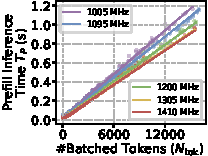
\includegraphics[width=\linewidth]{figs/ttft_vs_tokens.pdf}
        \caption{Prefill.}
        \label{fig:pred-ttft}
    \end{subfigure}
    \hfill
    \begin{subfigure}[b]{0.49\columnwidth}
        \centering

        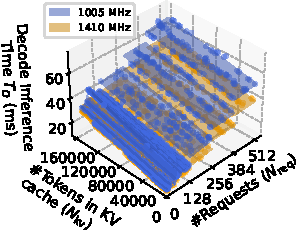
\includegraphics[width=\linewidth]{figs/itl-prediction.pdf}
        \caption{Decode.}
        \label{fig:pred-itl}
    \end{subfigure}
    \caption{Offline profiling results for LLaMA-3.1-8B on A100. Each point is a collected sample. Prefill latency grows near linearly with batched tokens, and decode latency exhibits tile-structured behavior across request numbers and KV-cache size. Lines and planes are visual guides to illustrate predictability. }
    \label{fig:pred-tile}
\end{figure}

\begin{figure}[!t]
    \centering
    \begin{minipage}[b]{0.40\columnwidth}
        \centering
        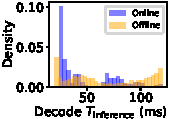
\includegraphics[width=\textwidth]{figs/dist_shift_itl.pdf}
        \caption{Distribution shift of decode model inference time between online and offline data.}
        % # Offline data are sampled uniformly in $(N_{\text{req}}, N_{\text{kv}})$.}
        \label{fig:dist-shift}
        % \jiahuan{redraw}
    \end{minipage}
    \hfill
    \begin{minipage}[b]{0.58\columnwidth}
        \centering
        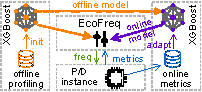
\includegraphics[width=\textwidth]{figs/voltanallm-design-feedback.drawio.pdf}
        \caption{Overview of \predictor. The inference time prediction model is initialized by offline profiling and continuously refined using online metrics, enabling accurate runtime model inference time prediction.}
        \label{fig:predictor}
    \end{minipage}
\end{figure}

To overcome such distribution shift, we propose \emph{online adaptation}.
As shown in \fref{fig:predictor}, before the deployment, \predictor first performs the offline profiling and model training to build the initial offline predictors $T_P^{\text{offline}}(\cdot)$ and $T_D^{\text{offline}}(\cdot)$.
During runtime, \predictor continuously collects online performance metrics and initiates a background finetuning process every $X$ new samples to produce the updated finetuned models $T_P^{\text{online}}(\cdot)$ and $T_D^{\text{online}}(\cdot)$.
This online finetuning allows \predictor to maintain accuracy despite the dynamic workload variations.

At runtime, \governor queries \predictor to estimate P/D model inference times.
Since the models are lightweight, this prediction incurs negligible overhead (e.g., $<$0.5 ms). 

\subsection{\router: State Space-Guided Routing} 
\label{subsec:router}

While \governor adaptively controls GPU frequency for energy efficiency, request routing offers another key opportunity for energy optimization in multi-instance systems.
% Although \eref{eq:formulation-routing-beg}–\ref{eq:formulation-routing-end} define the theoretical global optimal request routing, directly solving it is not feasible for online deployment. The problem is NP-hard with search space of $(\mathbf{I}^P_p, \mathbf{I}^D_d)$ and unknown requests arrival pattern (e.g., total request number $R$ is unknown).
% Instead of solving a global assignment problem, we reframe routing from the perspective of each decode instances' energy-latency \emph{state space}.

\noindent
\textbf{State-space perspective.}
As established earlier in \sref{subsec:predictor}, the ITL and energy consumption of a decode instance are functions of the triple $(N_{\text{req}}, N_{\text{kv}}, f)$.
Since \governor determines $f$ based on $(N_{\text{req}}, N_{\text{kv}})$, each instance's operating condition can be represented as a point in the $(N_{\text{req}}, N_{\text{kv}})$ state space.
% Each point in the space denotes a feasible operating state of this decode instance.
When requests arrive, finish, or generate new tokens, the instance moves to a different point in this state space. 
A visualization of this state space (\fref{fig:router-motivation}) shows the ``frequency cliff'' created by batch-size boundaries (\sref{subsec:tile-effect}). When $N_{\text{req}}$ crosses a batch size boundary (e.g., 256), ITL increases significantly, which forces \governor to raise frequency sharply to maintain SLOs. This produces a disproportionate jump in energy consumption. Therefore, an effective routing policy should try to keep instances away from these high-cost regions whenever possible. 
% The figure clearly reveals the frequency ``cliff'' associated with the batch size boundary effect (\sref{subsec:tile-effect}).
% When $N_{\text{req}}$ crosses a batch size boundary (e.g., 256), ITL increases significantly, compelling \governor to raise the frequency to ensure SLO attainment.

\begin{figure}[!t]
    \centering
    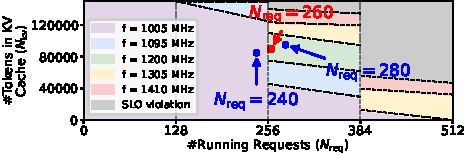
\includegraphics[width=\linewidth]{figs/sec-router-feasible-region.pdf}
    \caption{Example state space of a decode instance. The axes represent the number of running requests ($N_{\text{req}}$) and the number of tokens in KV cache ($N_{\text{kv}}$). Colored regions show the operating frequency $f$ chosen by \governor. The annotated points illustrate how different routing choices (e.g., $N_{\text{req}}=240, 260, 280$) place the instance in low- or high-frequency regions.}
    \label{fig:router-motivation}
\end{figure}

\noindent
\textbf{Motivating example.}
% From this state space perspective, request routing involves ``navigating'' the points of multiple decode instances in the state space.
% Intuitively, to conserve energy, this navigation should avoid the frequency ``cliff'' at batch size boundaries.
Consider 2 decode instances, 520 total requests, and a batch boundary at 256.
A ``symmetric'' router (red point in \fref{fig:router-motivation}) dispatching 260 requests to each instance forces both to cross the ``cliff'', compelling higher frequency to meet the SLO.
In contrast, an ``asymmetric'' routing decision (blue points in \fref{fig:router-motivation}) could assign 240 requests to one instance, keeping it below the ``cliff'' at a low frequency, while the other instance handles 280 requests, incurring a small, SLO-compliant ITL increase. Although slightly imbalanced, this assignment is more energy efficient overall. This illustrates why routing should consider where each instance lies in the state space, rather than treating all instances uniformly. 
% Consequently, this ``asymmetric'' routing strategy achieves higher energy efficiency.

% \jiahuan{can simplify to 2 cases if space is problem: merge case 1 and 3 to: round robin of $\min{\mathcal{F}^\prime}$}

\noindent
\textbf{State-space guided routing design.}
We propose \router to exploit this opportunity.
Instead of exhaustively searching for the optimal assignment, \router makes online routing decision when each decode request arrives.
Leveraging the concept of state space, \router performs a ``what-if'' analysis: it hypothetically assigns the request to \emph{all} instances, navigates their state spaces and evaluates frequency changes, then makes the routing decision.
The algorithm compares the \emph{current} frequencies $\mathcal{F}$ with the hypothetically \emph{resulting} frequencies $\mathcal{F}^\prime$, leading to the following cases:
\ding{202} \textbf{Partial instances increase the frequencies, and the spread of $\mathcal{F}^\prime$ remains within the threshold} ($\max(\mathcal{F}^\prime)-\min(\mathcal{F}^\prime) \le \Delta$).
\router selects the instance with the lowest \emph{unchanged} frequency.
This rule avoids unnecessarily crossing the previously discussed frequency ``cliff''.
\ding{203} \textbf{Other situations}, covering (a) no changes ($\mathcal{F}=\mathcal{F}^\prime$), (b) all instance increase the frequencies, and (c) partial instance increase the frequency, but $\max(\mathcal{F}^\prime)-\min(\mathcal{F}^\prime) > \Delta$.
\router selects the instance with the lowest resulting frequency ($\min(\mathcal{F}^\prime)$) using round-robin.
\appref{subsubsec:router-algo-blk} gives a formal detailed version of above algorithm, and \fref{fig:router-design} provides an illustration for a 2-instance system.
\cameraready{
It is noted that \router is also lightweight and does not introduce significant latency.
Its primary overhead comes from the latency prediction of \predictor, which takes $<$0.5 ms per query (\sref{subsec:predictor}).
Also, multiple queries for different decode instance candidates are batched together and processed by the underlying XGBoost model of \predictor to further minimize the latency.
Additionally, the routing algorithm itself relies on simple logic.
Consequently, \router introduces a negligible extra latency of $<$1 ms per request.
}


% \router selects the instance within those with lowest resulting frequency ($\min(\mathcal{F}^\prime)$) in a round-robin manner.

% \noindent
% \ding{202} \textbf{No frequency changes} ($\mathcal{F}=\mathcal{F}^\prime$).
% There are two sub-cases:
% \textbf{(a)} If all instances share the same frequency, the algorithm falls back to a round-robin policy.
% \textbf{(b)} Otherwise, it selects the instance with lowest current frequency ($\min(\mathcal{F})$).

% \noindent

% \noindent
% \ding{203} \textbf{Partial instances increase the frequencies}. 
% Let $\Delta$ be a frequency difference threshold.
% There are two sub-cases:
% \textbf{(a)} If the difference between lowest and highest resulting frequency is within the threshold ($\max(\mathcal{F}^\prime)-\min(\mathcal{F}^\prime) \le \Delta$), \router selects the instance with the lowest \emph{unchanged} frequency.
% This rule avoids unnecessarily crossing the previously discussed frequency ``cliff''.
% \textbf{(b)} Otherwise, \router selects the instance with the lowest resulting frequency ($\min(\mathcal{F}^\prime)$).
% This rule serves as a safeguard against severe load imbalance.

% \noindent
% \ding{204} \textbf{All instances increase the frequencies}. \router selects the instance with lowest resulting frequency ($\min(\mathcal{F}^\prime)$).



\begin{figure}[!t]
    \centering
    % 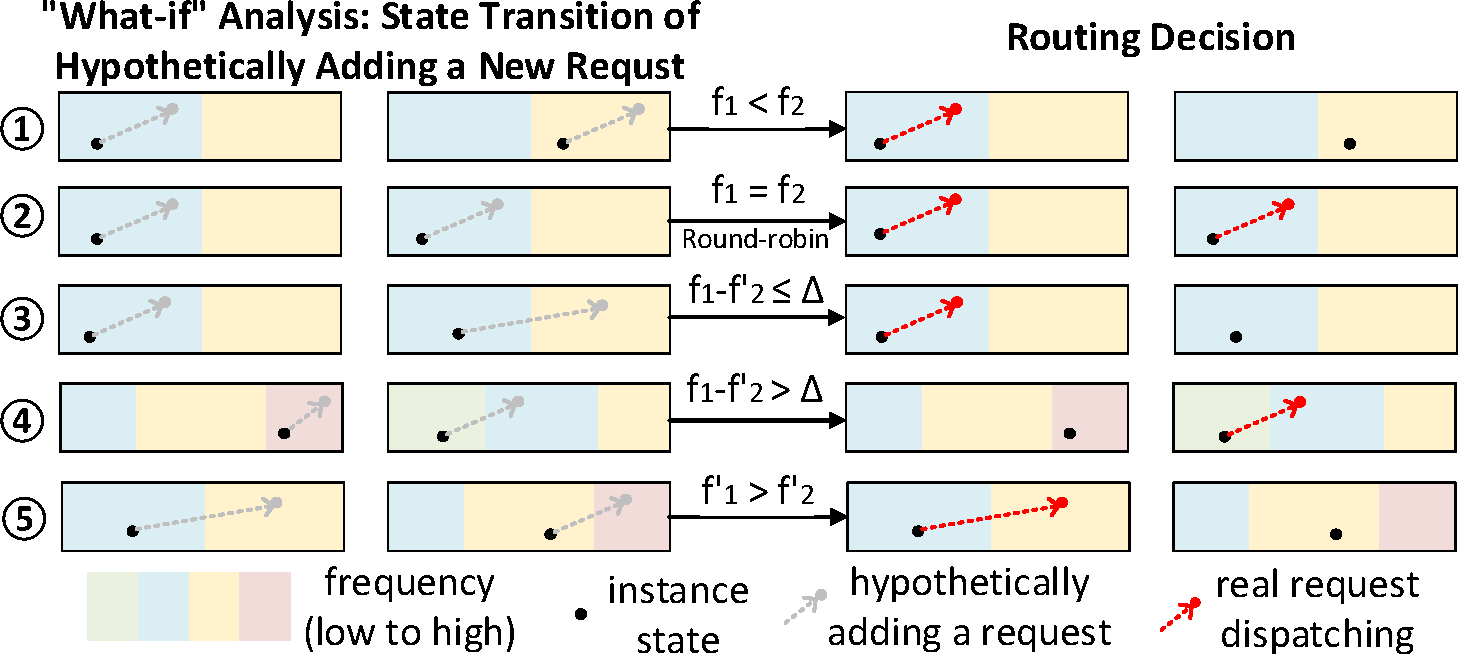
\includegraphics[width=\columnwidth]{figs/state-space.pdf}
    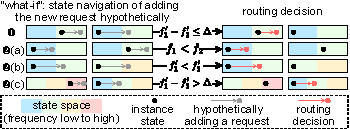
\includegraphics[width=\columnwidth]{figs/voltanallm-router.drawio.pdf}
    \caption{Illustration of \router for a system with 2 decode instances. Colors indicate the state space regions (mapped to different frequencies by \governor). The initial instance frequencies are $f_1$ and $f_2$, while $f^\prime_1$ and $f^\prime_2$ are the resulting frequencies after hypothetically adding the new request. \router evaluates these outcomes and selects the routing decision based on the corresponding decision rule (\ding{202}, \ding{203}a, \ding{203}b, \ding{203}c).}
    \label{fig:router-design}
\end{figure}

% \begin{algorithm}[!t]
%  \caption{\router: Decode Request Routing}
%  \label{alg:ecoroute}
%  \begin{algorithmic}[1]

%     \Require Decode instance list $\mathcal{D}=\{d_i\}_{i=1}^n$ and their state list $\mathcal{M}=\{m_i\}_{i=1}^n$, request for routing $r$, frequency decision of \governor $\freq(\cdot)$, frequency threshold $\Delta$.

%     \Ensure Selected decode instance $d\in\mathcal{D}$.

%     \State $\mathcal{F} \gets \{ \freq(m_i)\}_{i=1}^n$ \Comment{current freq of all instances}
%     \State $\mathcal{F}^\prime \gets \{ \freq(m_i \oplus r)\}_{i=1}^n$ \Comment{frequency after hypothetically adding request $r$, $\oplus$ denotes adding request}

%     \If{$\mathcal{F}=\mathcal{F}^\prime$} \Comment{\textbf{case \ding{202}}: no frequency changes}
%         \If{\Call{AllSame}{$\mathcal{F}$}} \Comment{\textbf{\ding{202}(a)}: all freqs are same}
%             \State \Return \Call{RoundRobin}{$\mathcal{D}$} \Comment{round-robin}
%         \Else  \Comment{\textbf{\ding{202}(b)}: not all same}
%             \State \Return $d_{\argmin_i \mathcal{F}}$ \Comment{min current freq}
%         \EndIf
%     \ElsIf{\Call{PartialChanged}{$\mathcal{F}$, $\mathcal{F}^\prime$}} \Comment{\textbf{case \ding{203}}: some frequencies increase}
%         \If{$\max(\mathcal{F}^\prime)-\min(\mathcal{F}^\prime) \le \Delta$}  \Comment{\textbf{\ding{203}(a)}: diff $\le\Delta$}
%             \State \Return $d_{\argmin_i \Call{Unchanged}{\mathcal{F}, \mathcal{F}^\prime}}$ \Comment{min unchanged}
%         \Else  \Comment{\textbf{\ding{203}(b)}: diff $>\Delta$}
%             \State \Return $d_{\argmin_i \mathcal{F}^\prime}$ \Comment{min resulting freq}
%         \EndIf
%     \EndIf
%     \State \Return $d_{\argmin_i \mathcal{F}^\prime}$  \Comment{\textbf{case \ding{204}}: all frequency increase}
%     % \Else \Comment{\textbf{case \ding{204}}: all frequencies increase}
%     %     \State \Return $d_{\argmin_i \mathcal{F}^\prime}$ \Comment{min resulting freq}
%     % \EndIf

%  \end{algorithmic}
% \end{algorithm}


% \begin{algorithm}[!t]
%  \caption{\router: Decode Request Routing}
%  \label{alg:ecoroute}
%  \begin{algorithmic}[1]

%     \Require Decode instance list $\mathcal{D}=\{d_i\}_{i=1}^n$ and their state list $\mathcal{M}=\{m_i\}_{i=1}^n$, request for routing $r$, frequency decision of \governor $\freq(\cdot)$, frequency threshold $\Delta$.

%     \Ensure Selected decode instance $d\in\mathcal{D}$.

%     \State $\mathcal{F} \gets \{ \freq(m_i)\}_{i=1}^n$ \Comment{current freq of all instances}
%     \State $\mathcal{F}^\prime \gets \{ \freq(m_i \oplus r)\}_{i=1}^n$ \Comment{frequency after hypothetically adding request $r$, $\oplus$ denotes adding request}

%     \If{\Call{PartialChanged}{$\mathcal{F}$, $\mathcal{F}^\prime$} $\And$ $\max(\mathcal{F}^\prime)-\min(\mathcal{F}^\prime) \le \Delta$}
%         \Statex /* \textbf{case} \ding{202}: if some but not all instances change the frequency, and the frequency difference $\le$ threshold */
%         \State \Return $d_{\argmin_i \Call{Unchanged}{\mathcal{F}, \mathcal{F}^\prime}}$ \Comment{min unchanged}
%     \EndIf
%     \Statex /* \textbf{case} \ding{203}: other situations */
%     \State \Return \Call{RoundRobin}{$d_{\argmin_i \mathcal{F}^\prime}$} \Comment{round-robin of min}

%     % \If{$\mathcal{F}=\mathcal{F}^\prime$} \Comment{\textbf{case \ding{202}}: no frequency changes}
%     %     \If{\Call{AllSame}{$\mathcal{F}$}} \Comment{\textbf{\ding{202}(a)}: all freqs are same}
%     %         \State \Return \Call{RoundRobin}{$\mathcal{D}$} \Comment{round-robin}
%     %     \Else  \Comment{\textbf{\ding{202}(b)}: not all same}
%     %         \State \Return $d_{\argmin_i \mathcal{F}}$ \Comment{min current freq}
%     %     \EndIf
%     % \ElsIf{\Call{PartialChanged}{$\mathcal{F}$, $\mathcal{F}^\prime$}} \Comment{\textbf{case \ding{203}}: some frequencies increase}
%     %     \If{$\max(\mathcal{F}^\prime)-\min(\mathcal{F}^\prime) \le \Delta$}  \Comment{\textbf{\ding{203}(a)}: diff $\le\Delta$}
%     %         \State \Return $d_{\argmin_i \Call{Unchanged}{\mathcal{F}, \mathcal{F}^\prime}}$ \Comment{min unchanged}
%     %     \Else  \Comment{\textbf{\ding{203}(b)}: diff $>\Delta$}
%     %         \State \Return $d_{\argmin_i \mathcal{F}^\prime}$ \Comment{min resulting freq}
%     %     \EndIf
%     % \EndIf
%     % \State \Return $d_{\argmin_i \mathcal{F}^\prime}$  \Comment{\textbf{case \ding{204}}: all frequency increase}
%     % \Else \Comment{\textbf{case \ding{204}}: all frequencies increase}
%     %     \State \Return $d_{\argmin_i \mathcal{F}^\prime}$ \Comment{min resulting freq}
%     % \EndIf

%  \end{algorithmic}
% \end{algorithm}

\fref{fig:router-example} conceptually illustrates how \router obtains energy benefits over a round-robin policy.
Round-robin suffers from the frequency ``cliff'' problem at batch size boundaries, like the ``symmetric'' router discussed before.
In contrast, \router is an ``asymmetric'' router, avoiding unnecessary frequency increases near the batch size boundaries.
Consequently, one instance (orange) operates for significantly more time at the energy-efficient low frequency than under the round-robin.



% \begin{figure}[!ht]
%     \centering
%     \begin{subfigure}[b]{0.49\columnwidth}
%         \centering
%         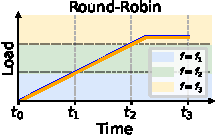
\includegraphics[width=\linewidth]{figs/sec-router-tile-aware.pdf}
%         \caption{Round-robin.}
%     \end{subfigure}
%     \begin{subfigure}[b]{0.49\columnwidth}
%         \centering
%         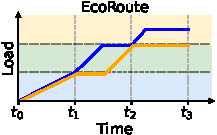
\includegraphics[width=\linewidth]{figs/sec-router-tile-aware-tile.pdf}
%         \caption{\router.}
%     \end{subfigure}    
%     \caption{Conceptual comparison of round-robin and \router with two decoding instances.
%     Line colors represent different instances. Shaded regions show the frequency levels required to meet SLOs ($f_1<f_2<f_3$). Under \router, one instance (orange) remains in a lower-frequency region for longer, yielding better energy efficiency than round-robin. }
%     \jiahuan{add figure tile, remove subfigure caption}
%     % \minjia{TODO: Can we move the legend down or adjust it a bit so it does not overlap with the curves in the left figure?}
%     % \jiahuan{done}
%     \label{fig:router-example}
% \end{figure}



While \router is effective for decode instances, we apply a simple round-robin policy for prefill instances for two reasons.
First, the prefill phase does not exhibit the significant batch size boundary effect seen in decode, as its batched token numbers are typically large (\sref{subsec:tile-effect} and \appref{appendix:prefill-tile}).
Second, the prefill phase is largely stateless, showing little system status correlation between consecutive batches (discussed in \fref{fig:prefill-tokens-fluctuation}).
Consequently, the state-space navigation approach used by \router is inapplicable to prefill.

\begin{figure}[!t]
    \centering
    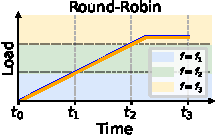
\includegraphics[width=0.49\columnwidth]{figs/sec-router-tile-aware.pdf}
    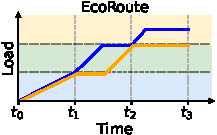
\includegraphics[width=0.49\columnwidth]{figs/sec-router-tile-aware-tile.pdf}
    \caption{Conceptual comparison of round-robin and \router with two decoding instances.
    Line colors represent different instances. Shaded regions show the frequency levels required to meet SLOs ($f_1<f_2<f_3$). Under \router, one instance (orange) remains in a lower-frequency region for longer, yielding better energy efficiency than round-robin. }
    % \jiahuan{add figure tile, remove subfigure caption}
    % \minjia{TODO: Can we move the legend down or adjust it a bit so it does not overlap with the curves in the left figure?}
    % \jiahuan{done}
    \label{fig:router-example}
\end{figure}


